% Project 3, Image Thresholding, ENEE612, UMBC, Professor Chang
% Author: Bernard Lampe

% Use the IEEE classes
\documentclass[journal]{IEEEtran}

% Packages
\usepackage[cmex10]{amsmath}
\usepackage{url}
\usepackage{cite}
\usepackage{graphicx}
\usepackage{subfig}
\usepackage{float}

% Correct bad hyphenation here
\hyphenation{op-tical net-works semi-conduc-tor}

% Start document
\begin{document}

% Paper title
\title{A Survey of Image Thresholding Techniques}

% Author
\author{Bernard~Lampe,~\IEEEmembership{Member,~IEEE}}

% The paper headers
\markboth{A Survey of Image Thresholding Techniques}%
{Shell \MakeLowercase{\Lampe}: A Survey of Image Thresholding Techniques}

% Make the title area
\maketitle

\begin{abstract}
In this paper, we survey two different approaches to non-parametric, gray-level image thresholding. The first approach computes a threshold as informed by the one dimensional histogram. This approach leverages the gray-level values solely to estimate an optimal threshold. We exemplified this approach by presenting results from three different algorithms which leverage the histogram in different ways. The second approach computes a threshold as informed by the gray-level values and the spatial correlations of those values in the image. This is accomplished by forming a two dimensional histogram which encodes the gray-levels as well as the spatial co-occurrences of those levels. As in the first approach, we present results of three different algorithms which take advantage of the spatial relationship of the pixels as represented by a two-dimensional histogram. Finally, this paper presents empirical results on a variety of different data sets. These data sets include portraits, natural scenes, medical and space-borne images. The goal is to give the reader an understanding of which techniques perform well in different imaging domains.
\end{abstract}

% Keywords
\begin{IEEEkeywords}
Thresholding, Histogram, Co-occurrence Matrix
\end{IEEEkeywords}

% Introduction with drop letter and first word capitalized.
\section{Introduction}
\IEEEPARstart{N}{on-parametric} thresholding of gray scale images is often an early step in image processing, analysis and understanding. Frequently, it is employed in image segmentation and object detection algorithms. The goal of thresholding algorithms is to assign each pixel of the image into one of two groups, foreground or background. The definition of foreground and background is domain specific, but in the general case, a white object on a black background will have a bi-model histogram. Any gray level between the modes of the histogram will obviously assign pixels of the object to the foreground and all others to the background. In practice, this simple example of a white object on a black background is not useful as most scenes contain objects which contain coincident gray scale values with the background or interact with the foreground and background. Shadows produced by the object and partially obscured objects are examples of these interactions. In these cases, finding the valley between the histogram modes may not be clear or computationally stable. Clearly, a more discriminating technique will be needed to choose an appropriate threshold which will minimize the error rate of pixel assignment. This analysis examines six such discriminating techniques which leverage different properties of the gray levels and spatial information besides the histogram shape.

% Introduction of one dimensional histogram based methods.
\subsection{Utilizing the One Dimensional Histogram}
\par The process of thresholding can be viewed as assigning pixels to one of two groups as described above. Therefore, many thresholding algorithms use the magnitude of the pixels themselves to compute an appropriate decision threshold. Here we purpose three different algorithms from existing literature which compute thresholds utilizing the pixel grayscale values. Each algorithm examined leverages the gray levels by first computing the one dimensional histogram.

\par First off, we examine the 1-bit Lloyd-Max quantizing algorithm \cite{lloyd} \cite{max}. The Lloyd-Max algorithm is a iterative, lossy, compression algorithm which aims to produce the best signal in a given number of bits. The criteria for best output signal was purposed by Max \cite{max} as a signal which minimizes the mean squared error (MSE) between the input and output probability mass functions (PMF) in the discrete case. This algorithm can be used to perform thresholding by compressing the pixels dynamic range from 8-bits to 1-bit, thereby attaining an image containing only two gray levels. The foreground can be assigned to the group which has the larger gray value label. This algorithm operates on the image histogram and converges to a solution which produces two groups which describe the histogram most accurately in a MSE sense. For example, if the histogram was bi-model, each mode would be in a separate group, and the group labels would be the grayscale values associated with the histogram modes. Another illustrative characterization of the 1-bit Lloyd-Max algorithm is that the pixels are quantized into one of two groups. Each group will have an equal area, or equal number of pixels, under the one dimensional function, the histogram, and the quantized labels will be the modes of each group. The iterative algorithm is described as follows below.

\begin{enumerate}
\item Compute an estimate of PMF using the histogram. \begin{math}p_i = n_i/N\end{math} where \begin{math}n_i\end{math} is the number of pixels with gray level \begin{math}i\end{math} and \begin{math}N\end{math} is the total number of pixels.
\item Divide the 8-bit grayscale dynamic range [0-255] into two equal sets by choosing a threshold \begin{math}k=128\end{math}.
\item For each set compute a representative value of each set \begin{math}y_i\end{math} as the centroid of the set members as in equation \ref{eq:lloydmaxcent}.
\item Compute a new threshold as the mid-point of the representative values of each set as in equation \ref{eq:lloydmaxmidpoint}.
\item For each set compute the distortion metric between the original PMF and the newly quantized PMF as in equation \ref{eq:lloydmaxmse}.
\item Repeat steps 3, 4 and 5 until the distortion measure no longer decreases.
\item Applying the quantized sets will result in a two level image.
\end{enumerate}

\begin{equation}
\label{eq:lloydmaxcent}
y_i = \frac{\sum{i p_i}}{\sum{p_i}}
\end{equation}

\begin{equation}
\label{eq:lloydmaxmidpoint}
k = \frac{y_{i+1}-y_i}{2}
\end{equation}

\begin{equation}
\label{eq:lloydmaxmse}
MSE_i=\sum(x_i-y_i)^2p_i
\end{equation}

\par Another, very prolific, thresholding method based on the gray-level values  is by Nobuyuki Otsu \cite{otsu}. This method assumes that within the distribution of gray level values there lies two classes which can be separated by an optimal threshold. The optimal threshold is the one which minimizes the within-class variance and maximizes between-class variance \cite{otsu}. Intuitively, we can say that the algorithm will choose the threshold which produces two classes which are as ``tight'' as possible and as ``far'' away from each other as possible. The algorithm proceeds by exhaustively searching all the possible thresholds [0-255] and at each hypothesized threshold, computes the objective function derived by Otsu and re-stated here in equation \ref{eq:otsuobj}. Finally, the threshold is chosen as the maximum of the objective function. The algorithm is described as follows.
\begin{enumerate}
\item Compute an estimate of PMF using the histogram. \begin{math}p_i = n_i/N\end{math} where \begin{math}n_i\end{math} is the number of pixels with gray level \begin{math}i\end{math} and \begin{math}N\end{math} is the total number of pixels.
\item For each possible threshold \begin{math}k\end{math} compute the value of the objective function as in equation \ref{eq:otsuobj}.
\item The optimal threshold \begin{math}k^*\end{math} is the max of the objective function as in equation \ref{eq:otsumax}.
\end{enumerate}

\begin{equation}
\mu(k) = \sum_{i=1}^{k}ip_i
\end{equation}

\begin{equation}
\omega(k) = \sum_{i=1}^{k}p_i
\end{equation}

\begin{equation}
\label{eq:otsuobj}
\sigma^2(k) = \frac{[\mu(255)\omega(k) - \mu(k)]^2}{\omega(k)[1-\omega(k)]}
\end{equation}

\begin{equation}
\label{eq:otsumax}
\sigma^2(k^*) = \max_{0<k<255} \sigma^2(k)
\end{equation}

\par The next thresholding algorithm also based on the one dimensional histogram is by T. Pun \cite{pun}. This method makes use of the definition of Shannon entropy of the histogram to compute an anisotropy coefficient. This coefficient is the percentage of the information which is present in the first half of the image pixels. This coefficient is used to threshold the image by assigning the gray-levels containing half the information to the background and the other pixels to the foreground. The goal is to choose a threshold such that each class of pixel contains as much of the image information as possible. The algorithm is described as follows.

\begin{enumerate}
\item Compute an estimate of PMF using the histogram. \begin{math}p_i = n_i/N\end{math} where \begin{math}n_i\end{math} is the number of pixels with gray level \begin{math}i\end{math} and \begin{math}N\end{math} is the total number of pixels.
\item Compute the anisotropy coefficient \begin{math}\alpha\end{math} as in equations \ref{eq:bpun} and \ref{eq:apun}.
\item The threshold \begin{math}k\end{math} is computed as in equation \ref{eq:tpun} below.
\end{enumerate}

\begin{equation}
\label{eq:bpun}
\sum_{i=0}^{na} p_i \approx \frac{1}{2}
\end{equation}

\begin{equation}
\label{eq:apun}
\alpha = \sum_{i=0}^{na} p_i log_2(p_i) / \sum_{i=0}^{255} p_i log_2(p_i)
\end{equation}

\begin{equation}
\label{eq:tpun}
\sum_{i=0}^{k} p_i = \frac{1}{2} + |\frac{1}{2} - \alpha|
\end{equation}

% Introduction of two dimensional histogram based methods.
\subsection{Utilizing the Two Dimensional Histogram}
\par In addition to the gray-levels of the pixels, images contain considerable information in the spatial correlation of adjacent pixels. This information can be leveraged to further improve the discriminating power of image thresholding algorithms. This information is especially relevant when the spatial interactions become more dominant than the gray-levels \cite{abutaleb}. For example, images that contain large amounts of noise and a low signal-to-noise ratio (SNR) exhibit considerable texture which can be exploited by examining the spatial correlations. Here we purpose three different algorithms from existing literature which compute thresholds from the pixel grayscale values and spatial information. Each algorithm examined represents the spatial information via co-occurrence relationships which count the number of times gray levels occur in adjacent pixels.

\par One of the earliest successful attempts to harness the spatial information of grayscale images in thresholding algorithms was developed by Abutaleb \cite{abutaleb}. Abutaleb's method computes a two dimensional co-occurrence histogram/matrix. The histogram counts are formed by the tuples of pixel gray-levels and the average of the adjacent pixel gray levels comprising the 8-connected neighborhood. The co-occurrence matrix captures the coincidences of pixel patterns, such as those seen in textures. This matrix is then normalized to form an estimate of the two dimensional probability mass function (PMF) of the two discrete random variables. After computation of the co-occurrence matrix, the threshold is computed by exhaustively searching over all the threshold tuples in the two dimensions and computing the maximum of the entropic objective function. This objective function is the sum of the entropy of the hypothesized foreground and background and is re-stated here in equations \ref{eq:asim} and \ref{eq:aobj}. By maximizing the objective function the threshold seeks to find a bi-level image which preserves the maximum amount of information in each class of pixels. The algorithm is described below.
\begin{enumerate}
\item Compute an estimate of joint PMF using the two dimensional histogram comprised of counts of the tuples of pixel gray levels and neighborhood averages. \begin{math}p_{ij} = f_{ij}/N\end{math} where \begin{math}f_{ij}\end{math} is the number of pixels with gray level \begin{math}i\end{math} and neighborhood average \begin{math}j\end{math}. Also \begin{math}N\end{math} is the total number of pixels.
\item Exhaustively search all tuples of possible thresholds \begin{math}(l,k)\end{math}. For each possible threshold tuple, divide the estimated joint PMF into four orthogonal regions as depicted in figure \ref{fig:abutaleb} and evaluate the entropic objective function as in equation \ref{eq:aobj}. Due to the assumption of pixel spatial correlation, two of the four regions of the PMF will be very sparse and only two will be considered in the objective function.
\item The optimal threshold will be the \begin{math}(l,k)\end{math} that are associated with the largest value of \begin{math}\psi \end{math}. Applying this threshold tuple to the histogram will produce a two level image where pixel falling in region D are classified as foreground pixels.
\end{enumerate}

\begin{figure}
\centering
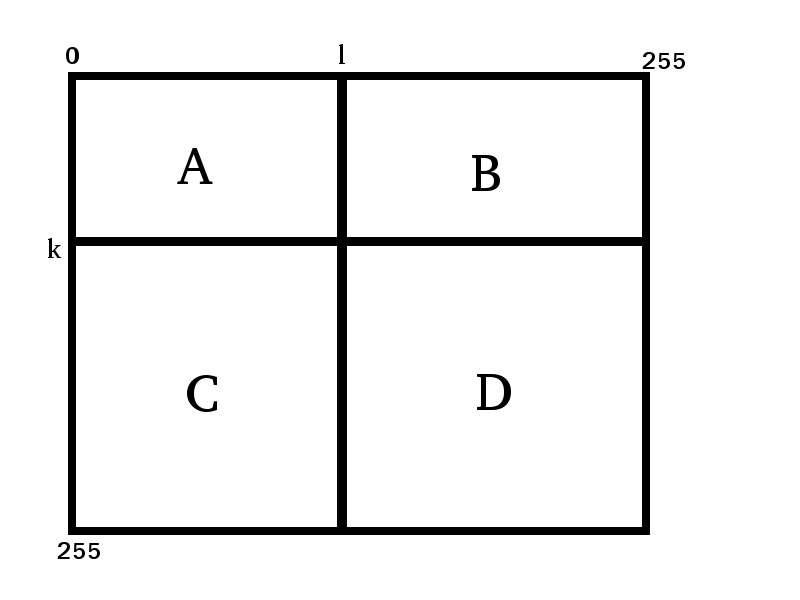
\includegraphics[width=3in]{./abutaleb.png}
\caption{Quandrants of Abutaleb's Co-occurrence Matrix at Threshold (l,k)}
\label{fig:abutaleb}
\end{figure}

\begin{equation}
\label{eq:asim}
\psi(l,k) = H(A) + H(D)
\end{equation}

\begin{equation}
P_{lk} = \sum_{i=1}^{l} \sum_{j=1}^{k} p_{ij}
\end{equation}

\begin{equation}
H_{lk} = - \sum_{i=1}^{l} \sum_{j=1}^{k} p_{ij} * log_2(p_{ij})
\end{equation}

\begin{multline}
\label{eq:aobj}
\psi(l,k) = log_2(P_{lk}(1-P_{lk})) + H_{lk}/P_{lk} + \\(H_{mm} - H_{lk}) / (1-P_{lk})
\end{multline}

\par Another image thresholding algorithm that leverages the spatial information was developed by Pal-Pal \cite{pal}. This algorithm computes the two dimensional co-occurrence histogram/matrix similar to Abutaleb's method. The histogram counts are formed by the tuples of pixel gray levels and the gray levels of the adjacent pixels in the 4-connected neighborhood. In practice, only two of the 4-connected neighborhood pixels are used to compute the histogram/matrix. This speeds computation and has been shown to have negligible effect on the final threshold chosen \cite{chang}. After computing the co-occurrence matrix, a single threshold is exhaustively searched and two objective functions are maximized. The threshold associated with the maximum of either objective function may be used for final thresholding. Both objective functions are the sum of entropies of the segmented co-occurrence matrix. The local entropy is defined as the sum of entropies computed from the regions of the thresholded co-occurrence matrix. These regions are the transitions within the hypothesized background and foreground. The joint entropy is defined as the sum of the entropies computed from the other regions of the thresholded co-occurrence matrix. These regions are the transitions between the foreground and background. The algorithm is described below.
\begin{enumerate}
\item Compute an estimate of joint PMF using the two dimensional histogram comprised of counts of the tuples of pixel gray levels and neighborhood gray levels. \begin{math}p_{ij} = f_{ij}/N\end{math} where \begin{math}f_{ij}\end{math} is the number of pixels with gray level \begin{math}i\end{math} and neighborhood gray level \begin{math}j\end{math}. Also \begin{math}N\end{math} is the total number of pixels.
\item Exhaustively search each threshold \begin{math}k\end{math}. For each threshold, divide the joint PMF into four orthogonal regions as depicted in figure \ref{fig:pal} and evaluate the two objective functions for joint entropy and local entropy re-stated in equations \ref{eq:pal_je} and \ref{eq:pal_le}.
\item The optimal threshold will be the \begin{math}k\end{math} associated with the max of either objective function. Applying the local entropy threshold will give a two level image that discriminate between foreground and background. Using the joint entropy threshold will result in identifying pixels which are transitions between foreground and background.
\end{enumerate}

\begin{figure}
\centering
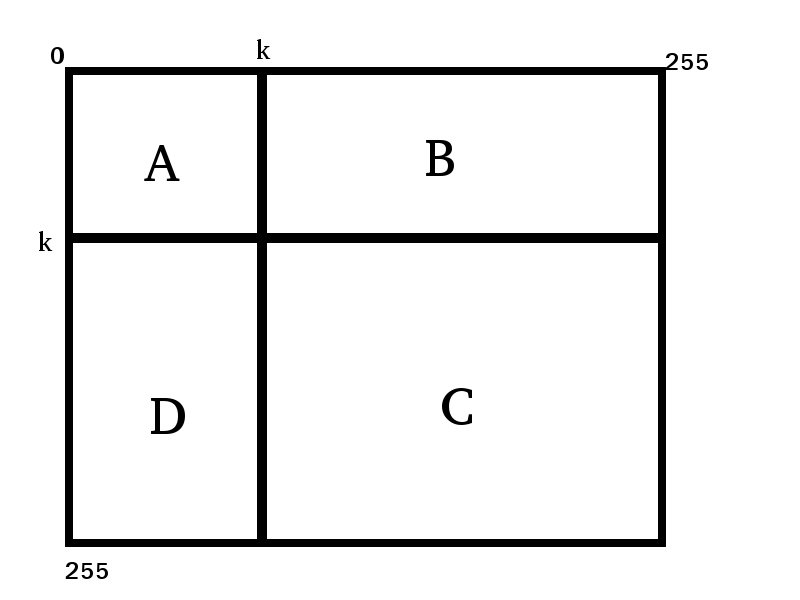
\includegraphics[width=3in]{./pal.png}
\caption{Quandrants of Pal's Co-occurrence Matrix at Threshold k}
\label{fig:pal}
\end{figure}

\begin{align}
p_{ij}^{A} &= p_{ij}/P_{A}(k), P_{A}(k) = \sum_{i=0}^k \sum_{j=0}^k p_{ij} \\
p_{ij}^{B} &= p_{ij}/P_{B}(k), P_{B}(k) = \sum_{i=0}^k \sum_{j=k+1}^{255} p_{ij} \\
p_{ij}^{C} &= p_{ij}/P_{C}(k), P_{C}(k) = \sum_{i=k+1}^{255} \sum_{j=k+1}^{255} p_{ij} \\
p_{ij}^{D} &= p_{ij}/P_{D}(k), P_{D}(k) = \sum_{i=k+1}^{255} \sum_{j=0}^{k} p_{ij}
\end{align}

\begin{equation}
\label{eq:pal_je}
H_{joint}^{(2)} = -\sum_{i=0}^{k} \sum_{j=k+1}^{255} p_{ij}^{B} log_2(p_{ij}^{B}) -
                   \sum_{i=k+1}^{255} \sum_{j=0}^{k} p_{ij}^{D} log_2(p_{ij}^{D})
\end{equation}

\begin{equation}
\label{eq:pal_le}
H_{local}^{(2)} = -\sum_{i=0}^{k} \sum_{j=0}^{k} p_{ij}^{A} log_2(p_{ij}^{A}) -
                   \sum_{i=k+1}^{255} \sum_{j=k+1}^{255} p_{ij}^{C} log_2(p_{ij}^{C})
\end{equation}

\par The last image thresholding algorithm examined also leverages the spatial information of the co-occurrence matrix and was developed by Chang et. al. \cite{chang}. The two dimensional co-occurrence histogram/matrix is computed as in the algorithm by Pal-Pal above. In addition, an exhaustive search of the possible image thresholds is conducted and a new objective function is maximized. The new objective function takes advantage of the entropy of all the segmented regions of the co-occurrence matrix to compute the relative entropy between the original image and the thresholded image. By using the relative entropy as an objective function, the algorithm computes the bi-level image which best represents the input image. The computation of the co-occurrence matrix and threshold searching are identical to the Pal-Pal algorithm above so only the new objective function will be given here in equation \ref{eq:chang}. In addition the region probabilities, such as \begin{math}P_A(k)\end{math} are computed as defined above in equations 15, 16, 17 and 18.

\begin{align}
p_{ij}^{'(A)}(k) = q_A(k) &= \frac{P_A(k)}{(k+1)(k+1)} \\
p_{ij}^{'(B)}(k) = q_B(k) &= \frac{P_B(k)}{(k+1)(255-k)} \\
p_{ij}^{'(C)}(k) = q_C(k) &= \frac{P_C(k)}{(255-k)(255-k)} \\
p_{ij}^{'(D)}(k) = q_D(k) &= \frac{P_D(k)}{(255-k)(k+1)}
\end{align}

\begin{multline}
\label{eq:chang}
\max L(p;p') = \sum_{i=0}^{255} \sum_{j=0}^{255}p_{ij}log_2(p_{ij}') = \\
P_A(k)log_2(q_A(k)) + P_B(k)log_2(q_B(k)) + \\ P_C(k)log_2(q_C(k)) + P_D(k)log_2(q_D(k))
\end{multline}

\section{Experiments}
\subsection{Image Data Set}
\par Images from different modalities were chosen to highlight the effectiveness of each thresholding algorithm. All images used were taken from those publicly available accompanying the Digital Image Processing Book by Gonzalez \cite{bworld}. The empirical analysis will take each data set in-turn and present the thresholded output produced from each algorithm.

\subsection{Application of Thresholding to Portrait}
\par The first data set considered is the famous portrait of Lena. The image is pictured in figure \ref{fig:lena}. This data set will give insight into how each of the thresholding algorithms perform on a typical portrait.

\begin{figure}[!h]
\centering
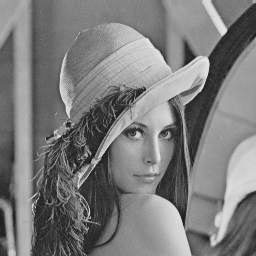
\includegraphics[width=3in]{../images/lena_gray_256.png}
\caption{Lena Original Image}
\label{fig:lena}
\end{figure}

\begin{table}[!h]
\centering
\begin{tabular}{cc}
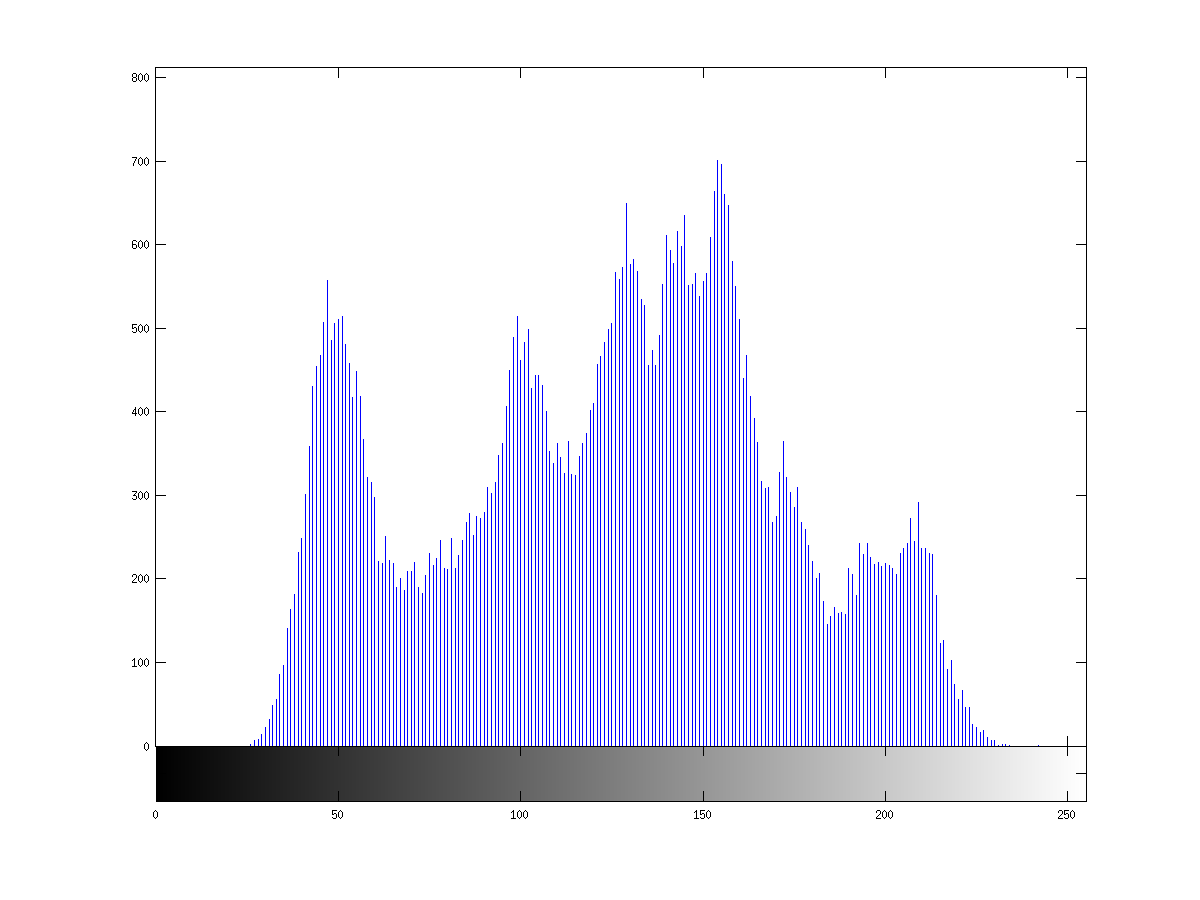
\includegraphics[width=1.5in]{../results/lena_gray_256_hist.png} &
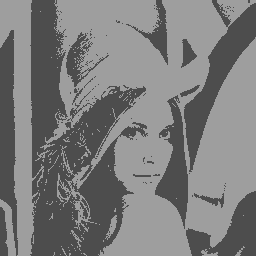
\includegraphics[width=1.5in]{../results/lena_gray_256_lloydmax.png} \\
\newline
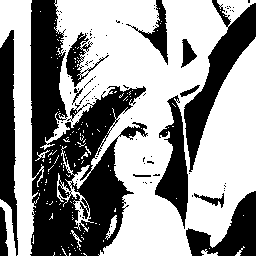
\includegraphics[width=1.5in]{../results/lena_gray_256_otsu.png} &
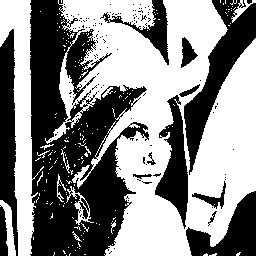
\includegraphics[width=1.5in]{../results/lena_gray_256_pun.png} \\
\end{tabular}
\caption{Top left: 1-D Histogram, Top right: Lloyd-Max (k=118), Bottom left: Otsu's (k=117), Bottom right: Pun's (k=125)}
\label{tab:lenaTable1}
\end{table}

\par Each of the one dimensional histogram thresholding algorithms was applied to the Lena image and the results are depicted in table \ref{tab:lenaTable1}. The captions are annotated with the thresholding values for each image. The algorithms of Lloyd-Max, Otsu and Pun all performed well on the portrait. Each was able to compute a threshold such that the shoulder, face and hat where classified as foreground. However, Pun's algorithm did slightly better at removing background pixels present directly above the hat.

\begin{table}[!h]
\centering
\begin{tabular}{cc}
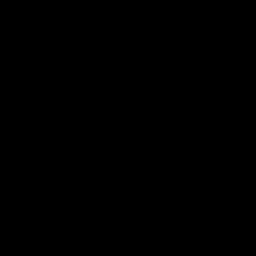
\includegraphics[width=1.5in]{../results/lena_gray_256_abutaleb.png} &
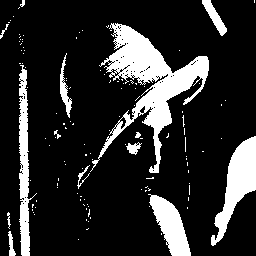
\includegraphics[width=1.5in]{../results/lena_gray_256_chang.png} \\
\newline
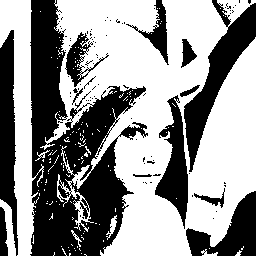
\includegraphics[width=1.5in]{../results/lena_gray_256_le_pal.png} &
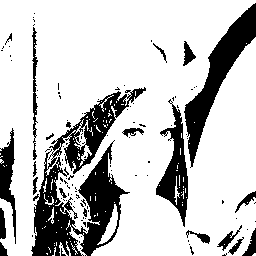
\includegraphics[width=1.5in]{../results/lena_gray_256_je_pal.png} \\
\end{tabular}
\caption{Top left: Abutaleb's (l,k=242,228), Top right: Chang's (k=170), Bottom left: Pal's Local Entropy (k=118), Bottom right: Pal's Joint Entropy (k=82)}
\label{tab:lenaTable2}
\end{table}

\par Next, each of the two dimensional histogram thresholding algorithms was applied to the Lena image and the results are in table \ref{tab:lenaTable2}. Upon examining the results, it is clear that the inclusion of spatial information in the thresholding process did not help in all cases. Abutaleb's method failed to identify any pixels as foreground. Pal's local entropy method produced results similar to the one dimensional histogram methods above. Pal's joint entropy method produced a threshold that is a little too high to discriminate some of the image features. Overall, Chang's method worked quite well in that it identified the hat, face and shoulder as foreground.

\subsection{Application of Thresholding to Outdoor Scene}
\par The next data set considered is the famous image known as Cameraman. The image is pictured in figure \ref{fig:cameraman}. This data set will give insight into how each of the thresholding algorithms perform on an outdoor scene.

\begin{figure}[!h]
\centering
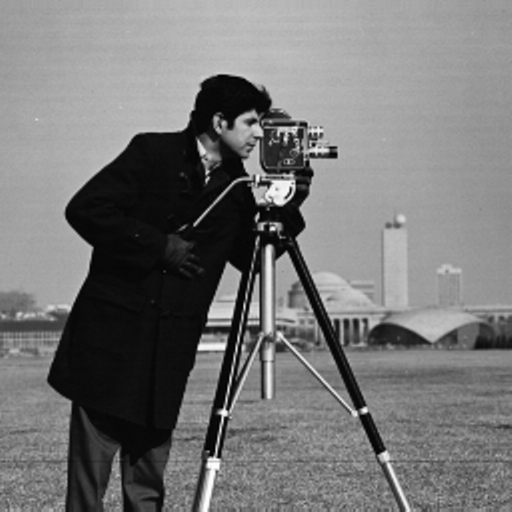
\includegraphics[width=3in]{../images/cameraman.png}
\caption{Cameraman Original Image}
\label{fig:cameraman}
\end{figure}

\begin{table}[!h]
\centering
\begin{tabular}{cc}
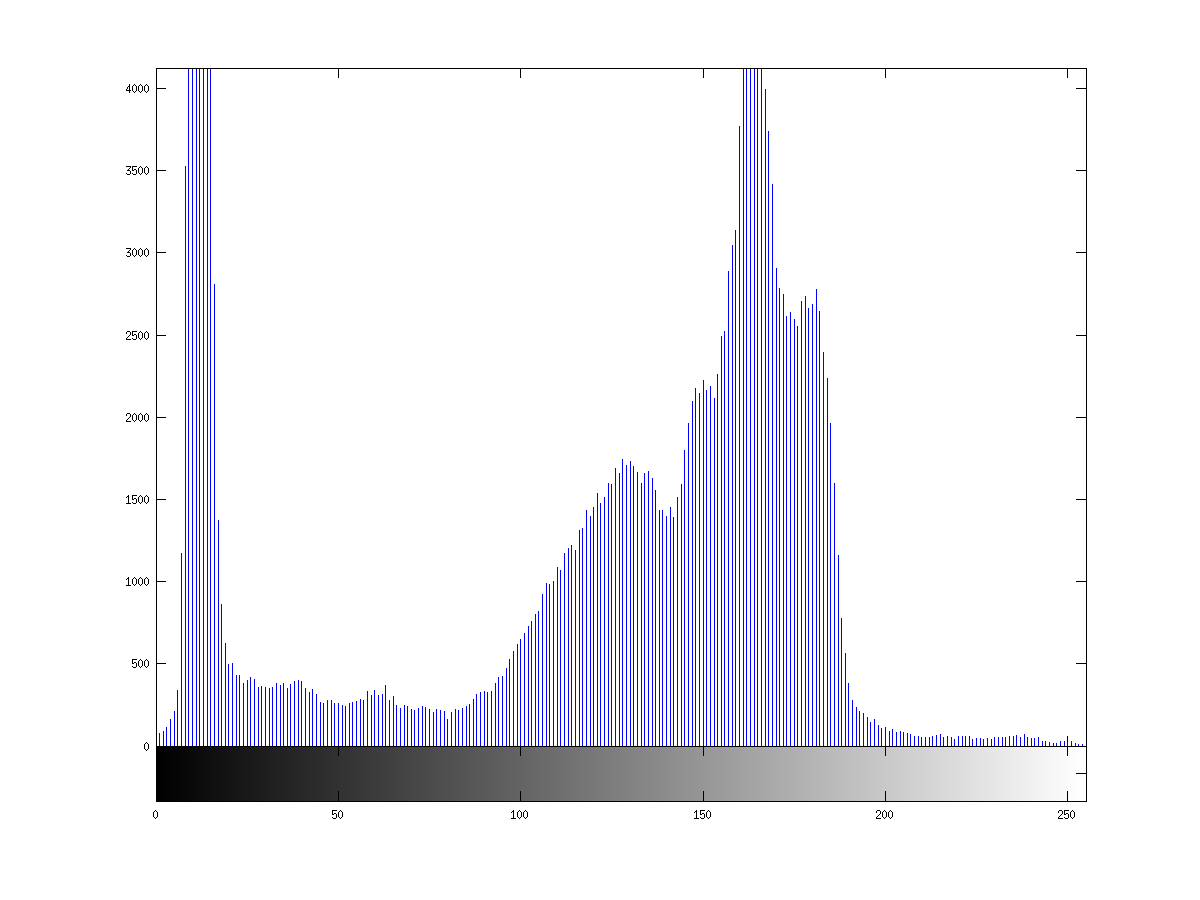
\includegraphics[width=1.5in]{../results/cameraman_hist.png} &
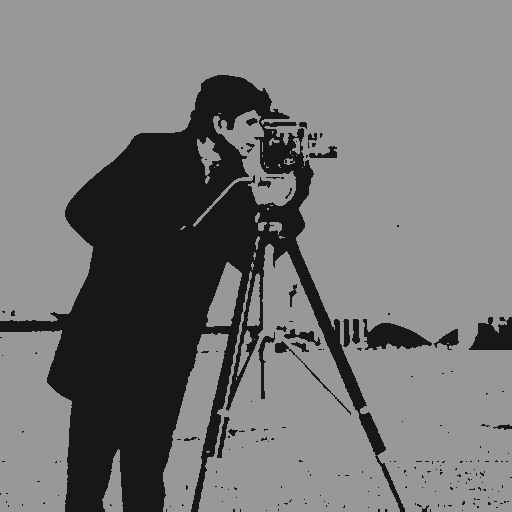
\includegraphics[width=1.5in]{../results/cameraman_lloydmax.png} \\
\newline
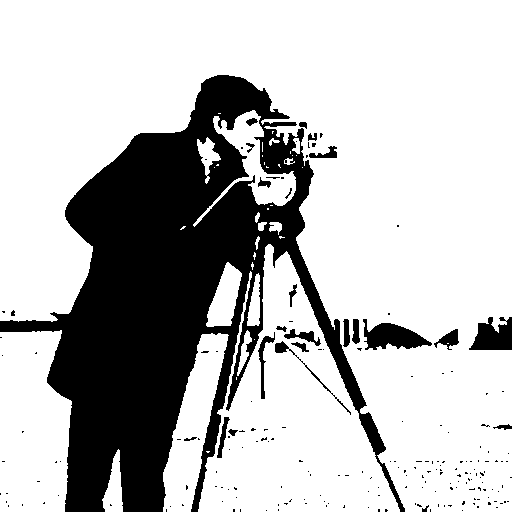
\includegraphics[width=1.5in]{../results/cameraman_otsu.png} &
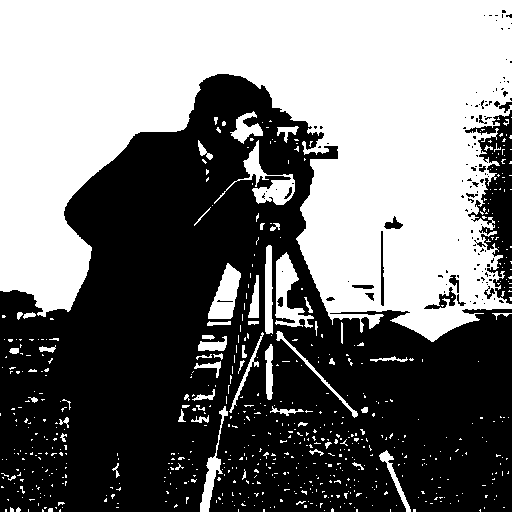
\includegraphics[width=1.5in]{../results/cameraman_pun.png} \\
\end{tabular}
\caption{Top left: 1-D Histogram, Top right: Lloyd-Max (k=88), Bottom left: Otsu's (k=87), Bottom right: Pun's (k=148)}
\label{tab:cameramanTable1}
\end{table}

\par Each of the one dimensional histogram thresholding algorithms was applied to the Cameraman image and the results are depicted in table \ref{tab:cameramanTable1}. The histogram is bi-modal with the scene background pixels consisting of the builds making up the histogram mode of the larger grayscale values. The algorithms of Lloyd-Max and Otsu performed equally well on the scene separating the background from the human figure and camera. Pun's algorithm did not perform as well in that many of the pixels of the grassy areas were classified with the human figure.

\begin{table}[!h]
\centering
\begin{tabular}{cc}
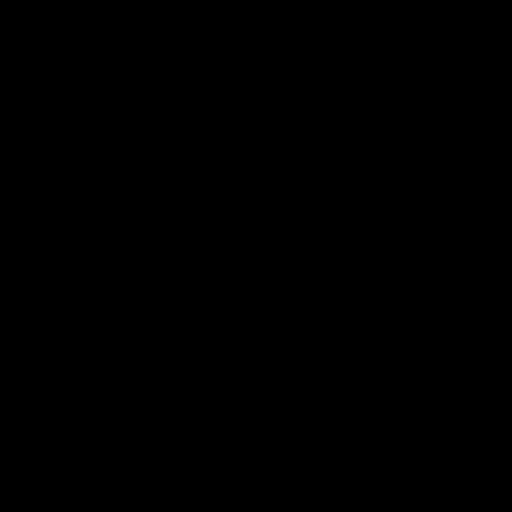
\includegraphics[width=1.5in]{../results/cameraman_abutaleb.png} &
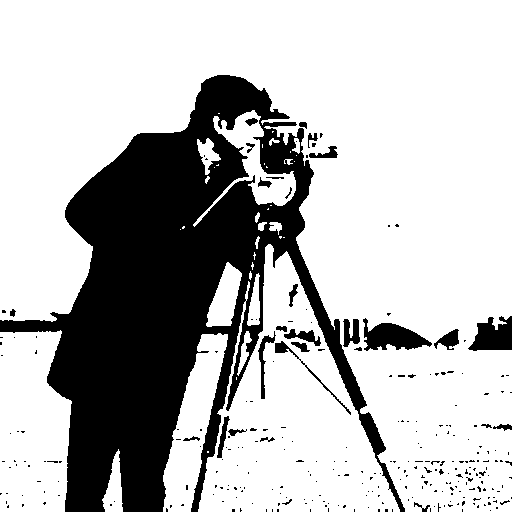
\includegraphics[width=1.5in]{../results/cameraman_chang.png} \\
\newline
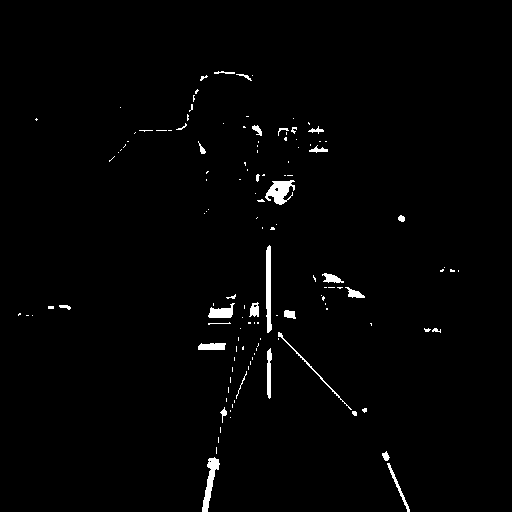
\includegraphics[width=1.5in]{../results/cameraman_le_pal.png} &
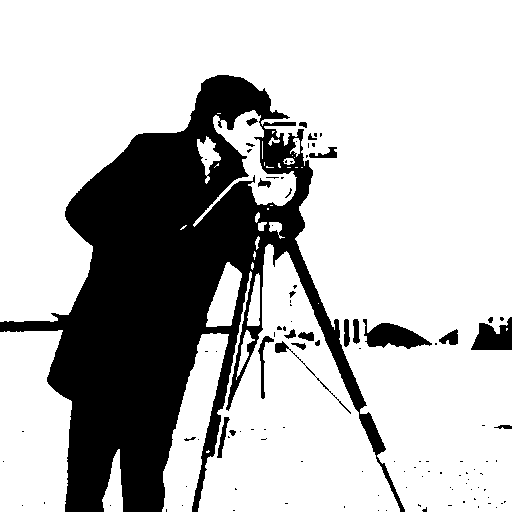
\includegraphics[width=1.5in]{../results/cameraman_je_pal.png} \\
\end{tabular}
\caption{Top left: Abutaleb's (l,k=254,252), Top right: Chang's (k=93), Bottom left: Pal's Local Entropy (k=193), Bottom right: Pal's Joint Entropy (k=80)}
\label{tab:cameramanTable2}
\end{table}

\par Next, each of the two dimensional histogram thresholding algorithms was applied to the Cameraman image and the results are in table \ref{tab:cameramanTable2}. The results show that the inclusion of spatial information in the thresholding process did not help in all cases. Again, Abutaleb's method failed to identify any pixels as foreground. Pal's local entropy method produced results which highlighted some of the edge features of the image. Pal's joint entropy method and Chang's method produced a threshold that is similar to Otsu's method giving good discrimination between the human figure with camera and the background buildings with grass.

\subsection{Application of Thresholding to Mammography Images}
\par The next data set considered is the mammography containing a large mass. The image is pictured in figure \ref{fig:breast}. This analysis will help determine which thresholding algorithm can discriminate the mass from the background.

\begin{figure}[!h]
\centering
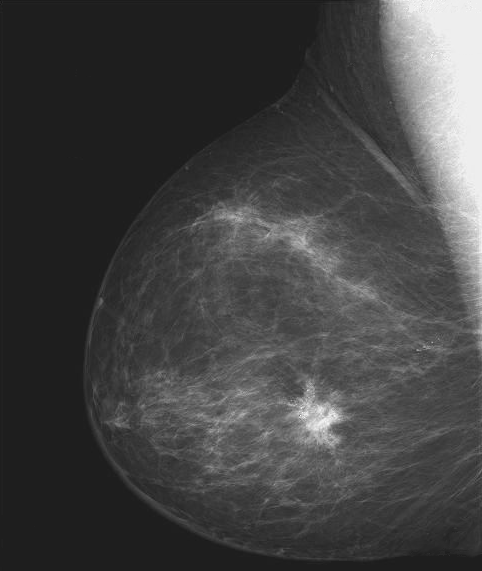
\includegraphics[width=3in]{../images/breast.png}
\caption{Original Mammography Image}
\label{fig:breast}
\end{figure}

\begin{table}[!h]
\centering
\begin{tabular}{cc}
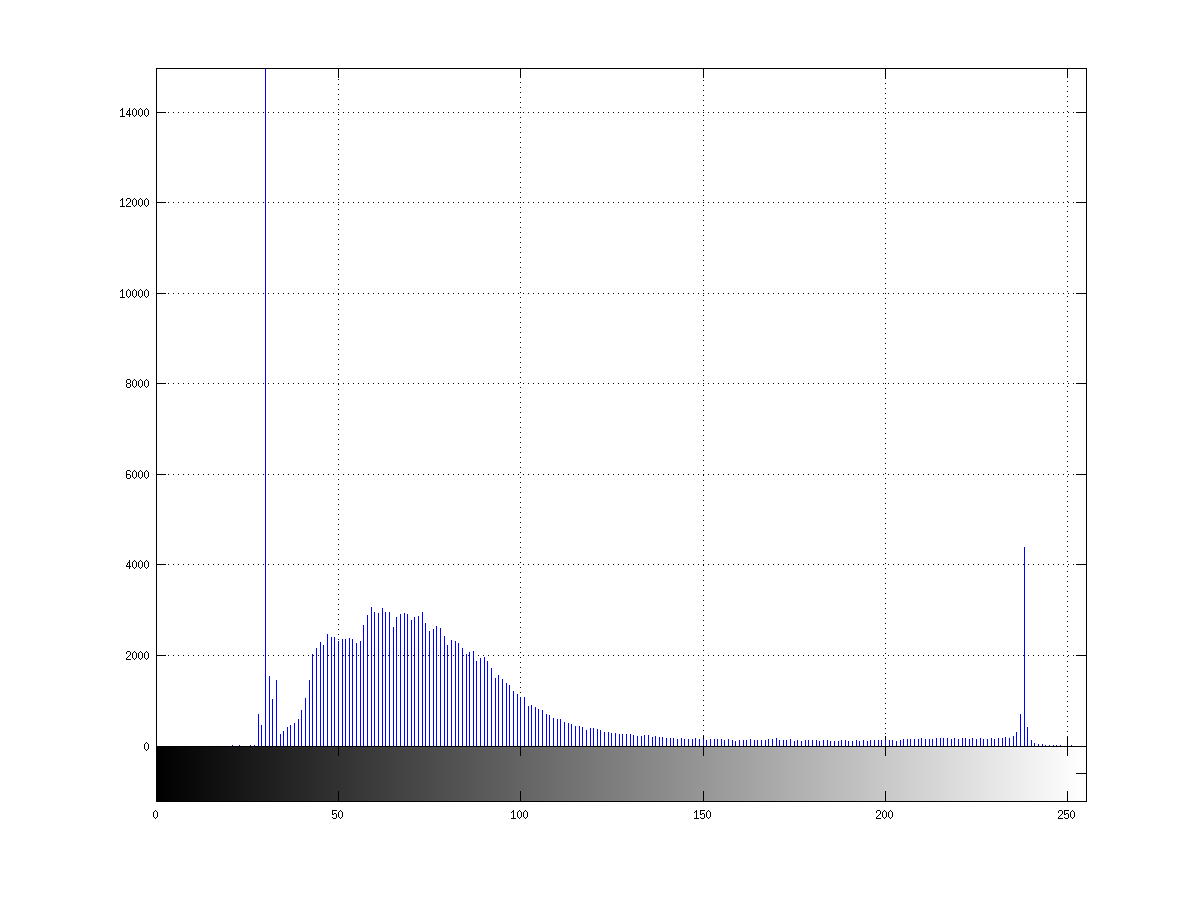
\includegraphics[width=1.5in]{../results/breast_hist.png} &
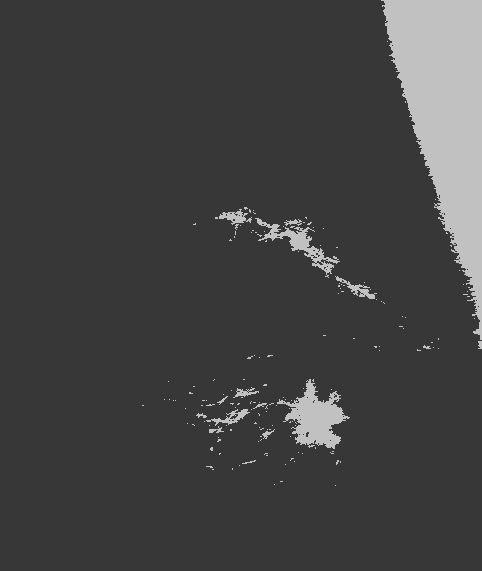
\includegraphics[width=1.5in]{../results/breast_lloydmax.png} \\
\newline
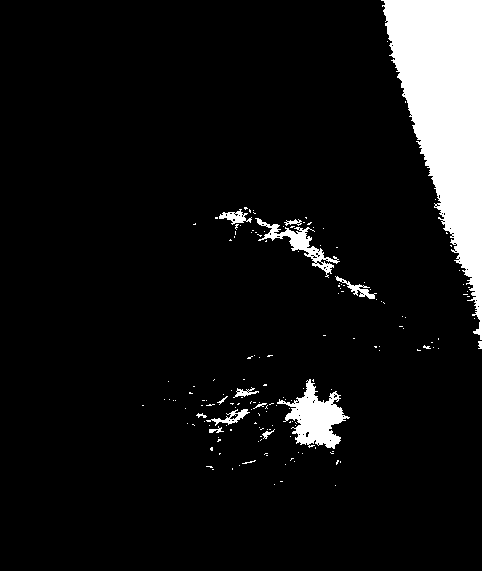
\includegraphics[width=1.5in]{../results/breast_otsu.png} &
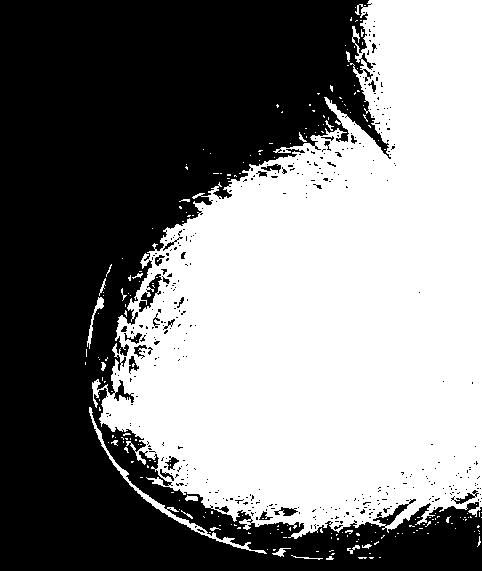
\includegraphics[width=1.5in]{../results/breast_pun.png} \\
\end{tabular}
\caption{Top left: 1-D Histogram, Top right: Lloyd-Max (k=124), Bottom left: Otsu's (k=124), Bottom right: Pun's (k=57)}
\label{tab:breastTable1}
\end{table}

\par Each of the one dimensional histogram thresholding algorithms was applied to the mammography image and the results are depicted in table \ref{tab:breastTable1}. The histogram has a large number of pixels at the extremes of the dynamic range. These are due to imaging artifacts from the background and saturation in the top right of the original image. The objects of interest are contained in the skewed log-normal distribution of the histogram. Evaluating the one dimensional histogram algorithms we see that the Lloyd-Max and Otsu's method were able to classify the two masses as foreground. However, Pun's method chose a threshold which was too low resulting in low discrimination of the mass.

\begin{table}[!h]
\centering
\begin{tabular}{cc}
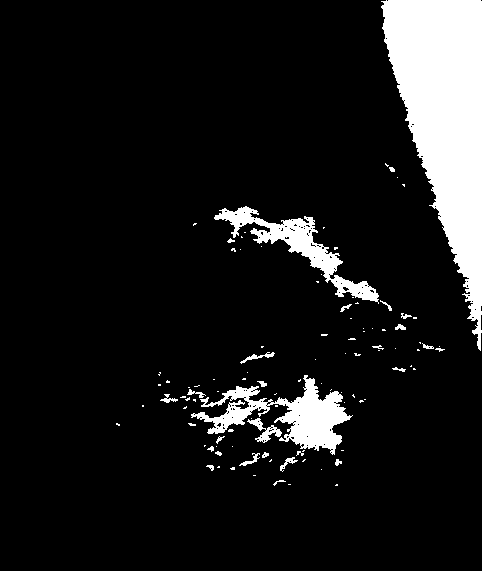
\includegraphics[width=1.5in]{../results/breast_abutaleb.png} &
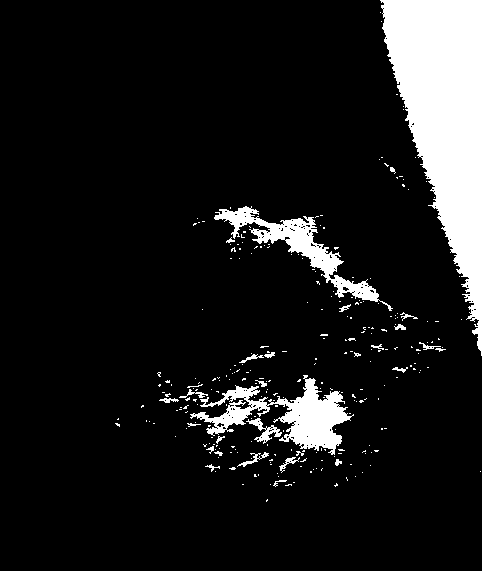
\includegraphics[width=1.5in]{../results/breast_chang.png} \\
\newline
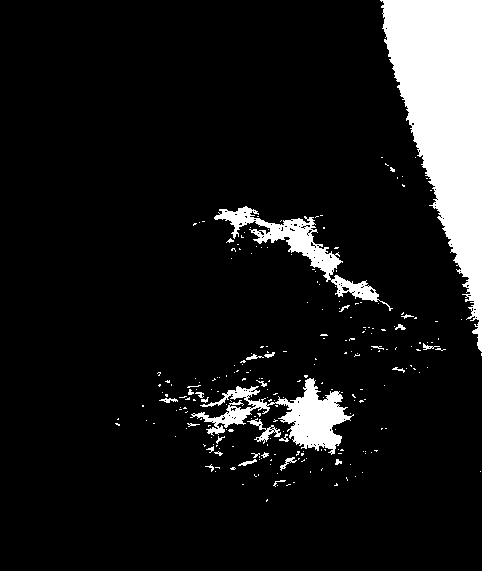
\includegraphics[width=1.5in]{../results/breast_le_pal.png} &
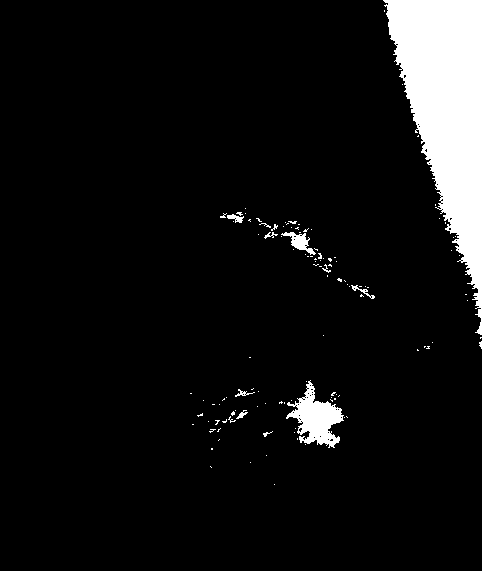
\includegraphics[width=1.5in]{../results/breast_je_pal.png} \\
\end{tabular}
\caption{Top left: Abutaleb's (l,k=108,107), Top right: Chang's (k=110), Bottom left: Pal's Local Entropy (k=111), Bottom right: Pal's Joint Entropy (k=136)}
\label{tab:breastTable2}
\end{table}

\par Next, each of the two dimensional histogram thresholding algorithms was applied to the mammography image and the results are in table \ref{tab:breastTable2}. Abutaleb's, Chang's and Pal's local entropy method all performed well on this image. They computed a threshold slightly lower than the previous algorithms and therefore classified more of the pixels from the mass as foreground. Pal's joint entropy method performed slightly worse than all the others, but was still able to isolate the mass.

\subsection{Application of Thresholding to Gamma Ray Imagery}
\par The next data set considered is an image created via gamma ray detection from the Crab pulsar in space. The image is pictured in figure \ref{fig:gamma}. This analysis will help determine which thresholding algorithm can discriminate the large emitting objects from the rest of the pulsar in the noisy image.

\begin{figure}[!h]
\centering
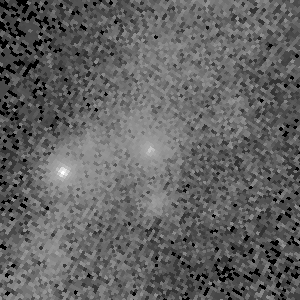
\includegraphics[width=3in]{../images/crabpulsar-gamma.png}
\caption{Original Crab Pulsar Gamma Image}
\label{fig:gamma}
\end{figure}

\begin{table}[!h]
\centering
\begin{tabular}{cc}
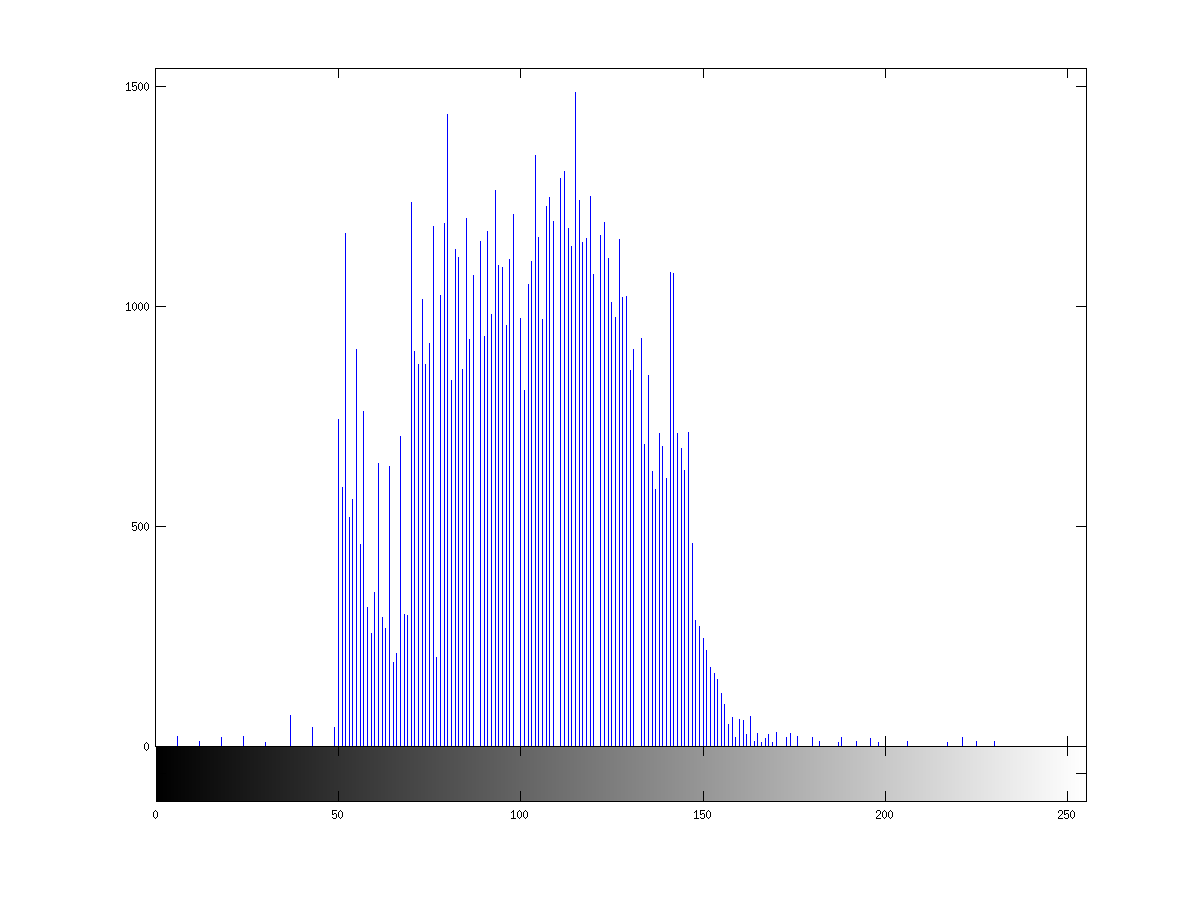
\includegraphics[width=1.5in]{../results/crabpulsar-gamma_hist.png} &
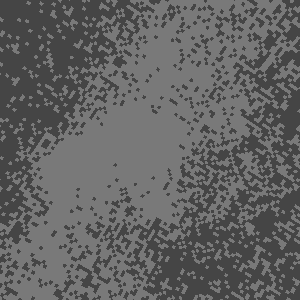
\includegraphics[width=1.5in]{../results/crabpulsar-gamma_lloydmax.png} \\
\newline
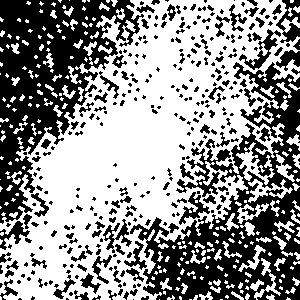
\includegraphics[width=1.5in]{../results/crabpulsar-gamma_otsu.png} &
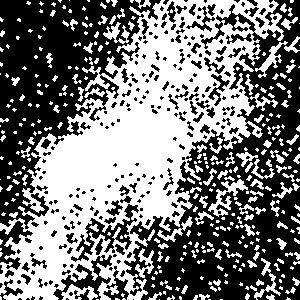
\includegraphics[width=1.5in]{../results/crabpulsar-gamma_pun.png} \\
\end{tabular}
\caption{Top left: 1-D Histogram, Top right: Lloyd-Max (k=95), Bottom left: Otsu's (k=94), Bottom right: Pun's (k=104)}
\label{tab:gammaTable1}
\end{table}

\par Each of the one dimensional histogram thresholding algorithms was applied to the Crab pulsar gamma image and the results are depicted in table \ref{tab:gammaTable1}. The Lloyd-Max and Otsu's algorithm performed identically while Pun's algorithm did slightly better. However, none of the algorithms were able to isolate the bright objects in the scene. Examining the one dimensional histogram does not give any insight as to where a good threshold would exist.

\begin{table}[!h]
\centering
\begin{tabular}{cc}
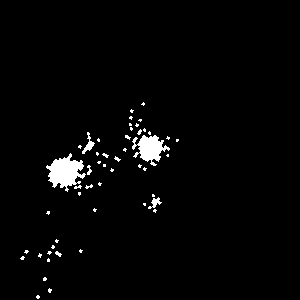
\includegraphics[width=1.5in]{../results/crabpulsar-gamma_abutaleb.png} &
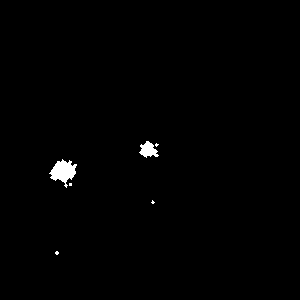
\includegraphics[width=1.5in]{../results/crabpulsar-gamma_chang.png} \\
\newline
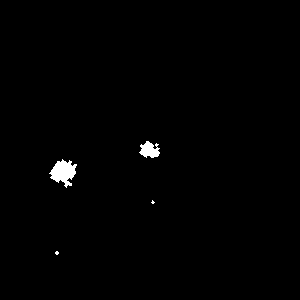
\includegraphics[width=1.5in]{../results/crabpulsar-gamma_le_pal.png} &
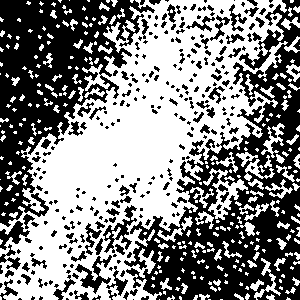
\includegraphics[width=1.5in]{../results/crabpulsar-gamma_je_pal.png} \\
\end{tabular}
\caption{Top left: Abutaleb's (l,k=148,95), Top right: Chang's (k=158), Bottom left: Pal's Local Entropy (k=156), Bottom right: Pal's Joint Entropy (k=99)}
\label{tab:gammaTable2}
\end{table}

\par Next, each of the two dimensional histogram thresholding algorithms was applied to the Crab pulsar gamma image and the results are in table \ref{tab:gammaTable2}. Abutaleb's, Chang's and Pal's local entropy algorithms were all able to discriminate the bright objects in the scene. Abutaleb's algorithm did slightly better at classifying more pixels from the bright objects when compared to Change and Pal's local entropy method. However, Abutaleb's algorithm does have more false alarms when compared to Chang and Pal's local entropy method. Pal's joint entropy method performed similarly to the one dimensional algorithms. Clearly, when taking into account the spatial information, i.e. texture, it is possible to determine a good threshold which isolates the bright objects of the scene.

\subsection{Application of Thresholding to Xray Imagery}
\par The last data set considered in this analysis is an image created via xray detection from the Crab pulsar in space. The image is pictured in figure \ref{fig:xray}. This image will give insight as to which thresholding algorithm can discriminate the large emitting objects from the rest of the pulsar.

\begin{figure}[!h]
\centering
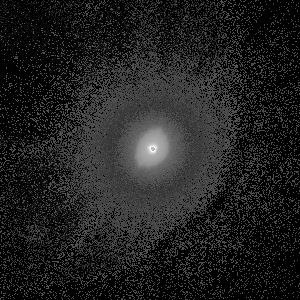
\includegraphics[width=3in]{../images/crabpulsar-xray.png}
\caption{Original Crab Pulsar Xray Image}
\label{fig:xray}
\end{figure}

\begin{table}[!h]
\centering
\begin{tabular}{cc}
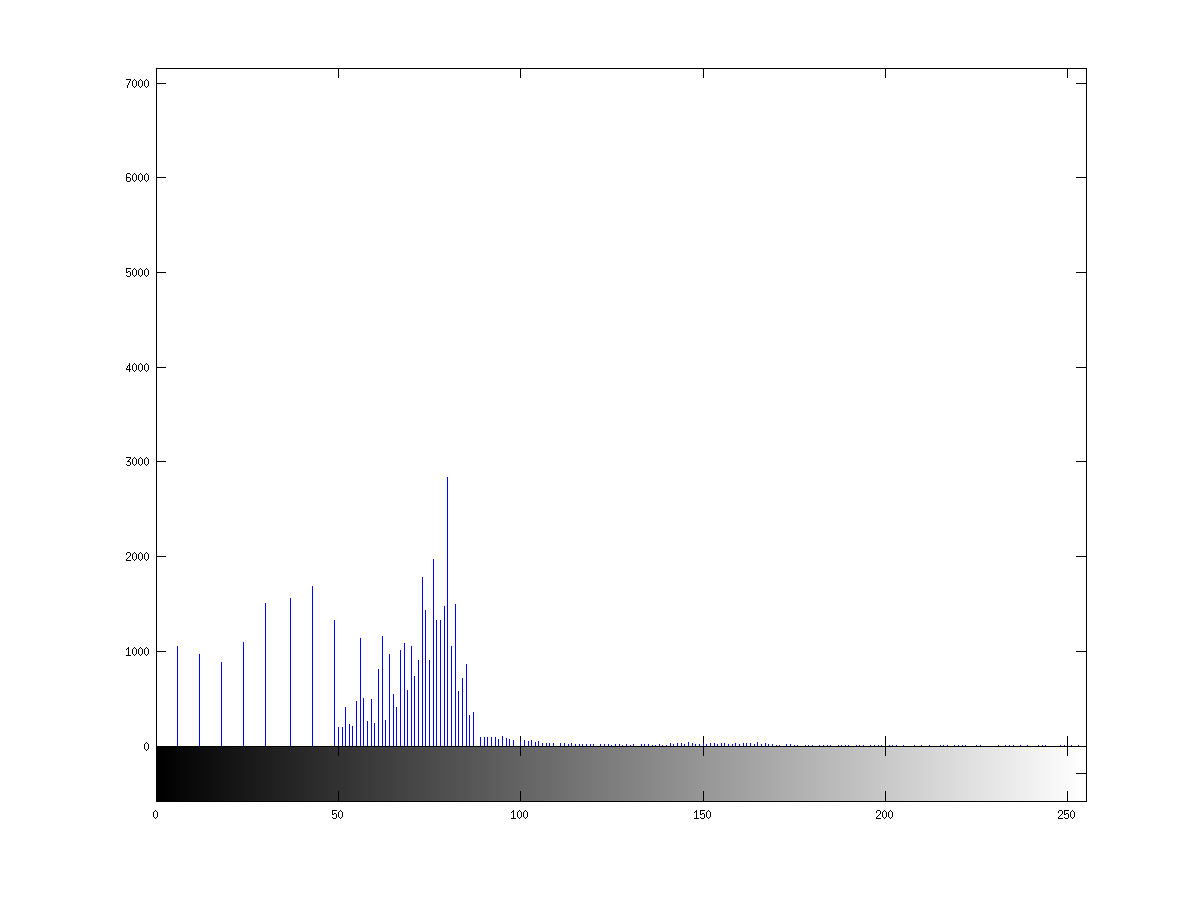
\includegraphics[width=1.5in]{../results/crabpulsar-xray_hist.png} &
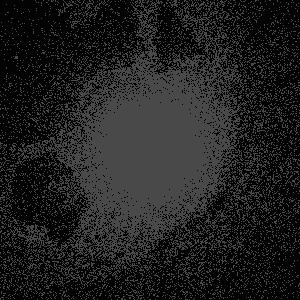
\includegraphics[width=1.5in]{../results/crabpulsar-xray_lloydmax.png} \\
\newline
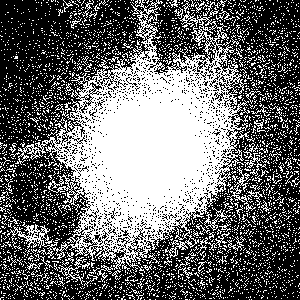
\includegraphics[width=1.5in]{../results/crabpulsar-xray_otsu.png} &
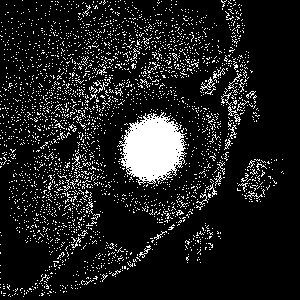
\includegraphics[width=1.5in]{../results/crabpulsar-xray_pun.png} \\
\end{tabular}
\caption{Top left: 1-D Histogram, Top right: Lloyd-Max (k=38), Bottom left: Otsu's (k=40), Bottom right: Pun's (k=80)}
\label{tab:xrayTable1}
\end{table}

\par Each of the one dimensional histogram thresholding algorithms was applied to the Crab pulsar xray image and the results are depicted in table \ref{tab:xrayTable1}. Again, the Lloyd-Max algorithm performed similarly to the Otsu's method. Also, Pun's method did better than Lloyd-Max and Otsu's method in discriminating the bright object at the center of the image. None of these method's did well in suppressing false alarms. Upon examining the histogram, it is not bi-modal and there does not appear to be an obvious separation of the pixels into clear object classes.

\begin{table}[!h]
\centering
\begin{tabular}{cc}
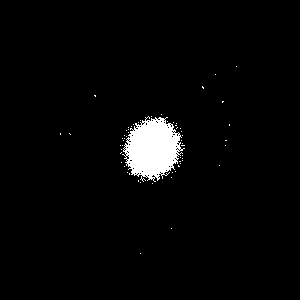
\includegraphics[width=1.5in]{../results/crabpulsar-xray_abutaleb.png} &
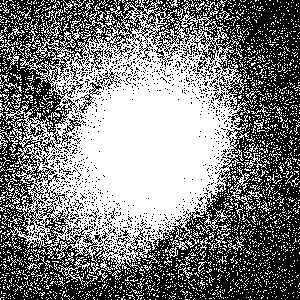
\includegraphics[width=1.5in]{../results/crabpulsar-xray_chang.png} \\
\newline
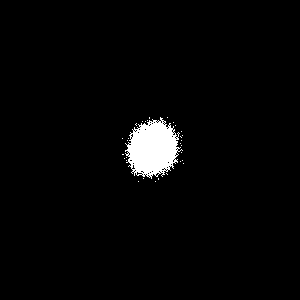
\includegraphics[width=1.5in]{../results/crabpulsar-xray_le_pal.png} &
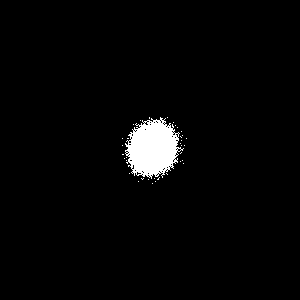
\includegraphics[width=1.5in]{../results/crabpulsar-xray_je_pal.png} \\
\end{tabular}
\caption{Top left: Abutaleb's (l,k=85,72), Top right: Chang's (k=2), Bottom left: Pal's Local Entropy (k=90), Bottom right: Pal's Joint Entropy (k=89)}
\label{tab:xrayTable2}
\end{table}

\par Next, each of the two dimensional histogram thresholding algorithms was applied to the Crab pulsar xray image and the results are in table \ref{tab:xrayTable2}. Abutaleb's, and both of Pal's methods performed well on this image in that they were able to isolate the bright object from the rest of the image. Chang's algorithm did not perform well on this particular data set.

\section{Conclusion}
This paper examined six different thresholding algorithms commonly used to threshold grayscale images. None of the algorithms performed well in all cases. Otsu's method and the Lloyd-Max algorithm performed almost identically on all images. In addition, using the co-occurrence matrix was not advantageous in all cases. In cases there were no dominant textures, leveraging the co-occurrence matrix degraded performance as seen in the Lena and Cameraman images. However, in cases were spatial interactions between pixels present high levels of texture, the co-occurrence matrix provided necessary information to the thresholding algorithm which allowed for better discrimination of objects in the scene. This was exemplified in the mammography image and space-borne images. The choice of a thresholding algorithm needs to be informed by the data on which it is operating. Inclusion of spatial information can degrade performance in cases of low texture, or can provide very powerful discrimination in cases of high texture.

% References section
\nocite{*}
\bibliographystyle{plain}
\bibliography{./references}

% Biography
\begin{IEEEbiographynophoto}{Bernard Lampe}
(M'09) became an IEEE Member (M) in 2009 and received his bachelors of science degree from The University of Michigan in Ann Arbor, Michigan, USA in 2009.
\par Mr. Lampe is also a member of the American Society for Computing Machines (ACM) since 2009.
\end{IEEEbiographynophoto}

% End document
\end{document}

